\documentclass[10pt]{article}
\usepackage[a4paper,landscape,margin=0.72in]{geometry}
\usepackage[T1]{fontenc}
\usepackage{lmodern,amsmath,amssymb,graphicx,hyperref}
\title{Weighted-Proj integrality: a checked prerequisite and open gluing gate}
\author{Bounded formal proof investigation}
\date{28 October 2026}
\begin{document}
\maketitle
\noindent The new Lean theorem proves that the infinity chart coordinate $\bar z$ is nonzero for every field and coefficient tuple. It does not prove that the whole weighted-$\operatorname{Proj}$ curve is integral, construct its global function field, or establish a divisor/Picard or compiled-runtime statement.

\section*{Checked result}
\texttt{WeightedProjIntegral.infinity\_chart\_z\_ne\_zero} uses the checked relation $\bar w^2=\bar z\bar u$ and the checked fact $\bar w\ne0$. Pinned Lean 4.34.1 exited zero; direct axiom output is \texttt{[propext, Classical.choice, Quot.sound]}. The exact source and compile output accompany this report.

\section*{Remaining proof bridge}
Existing proofs give a two-basic-open cover by the $X$ and $Z$ opens, an unconditional domain for the infinity chart, and a domain for the affine chart when the quintic is separable. The new nonzero result is a prerequisite for finding a point of $D(\bar z)$ in the infinity-chart spectrum. The missing checked step transports that point through the chart isomorphism and identifies it as lying in the actual $Z$-open of weighted $\operatorname{Proj}$. Without a nonempty intersection, two domain opens may form a disconnected reducible union.

After that transport, pinned Mathlib's \texttt{PreirreducibleSpace.of\_isOpenCover}, \texttt{IsReduced.of\_openCover}, and \texttt{isIntegral\_of\_irreducibleSpace\_of\_isReduced} provide a route to the whole-curve instance. This route is a dependency analysis; its conclusion is open. The CSV records the exact status of each step. No DLP experiments or cost measurements were run.

\clearpage
\section*{Proof dependencies}
\begin{center}
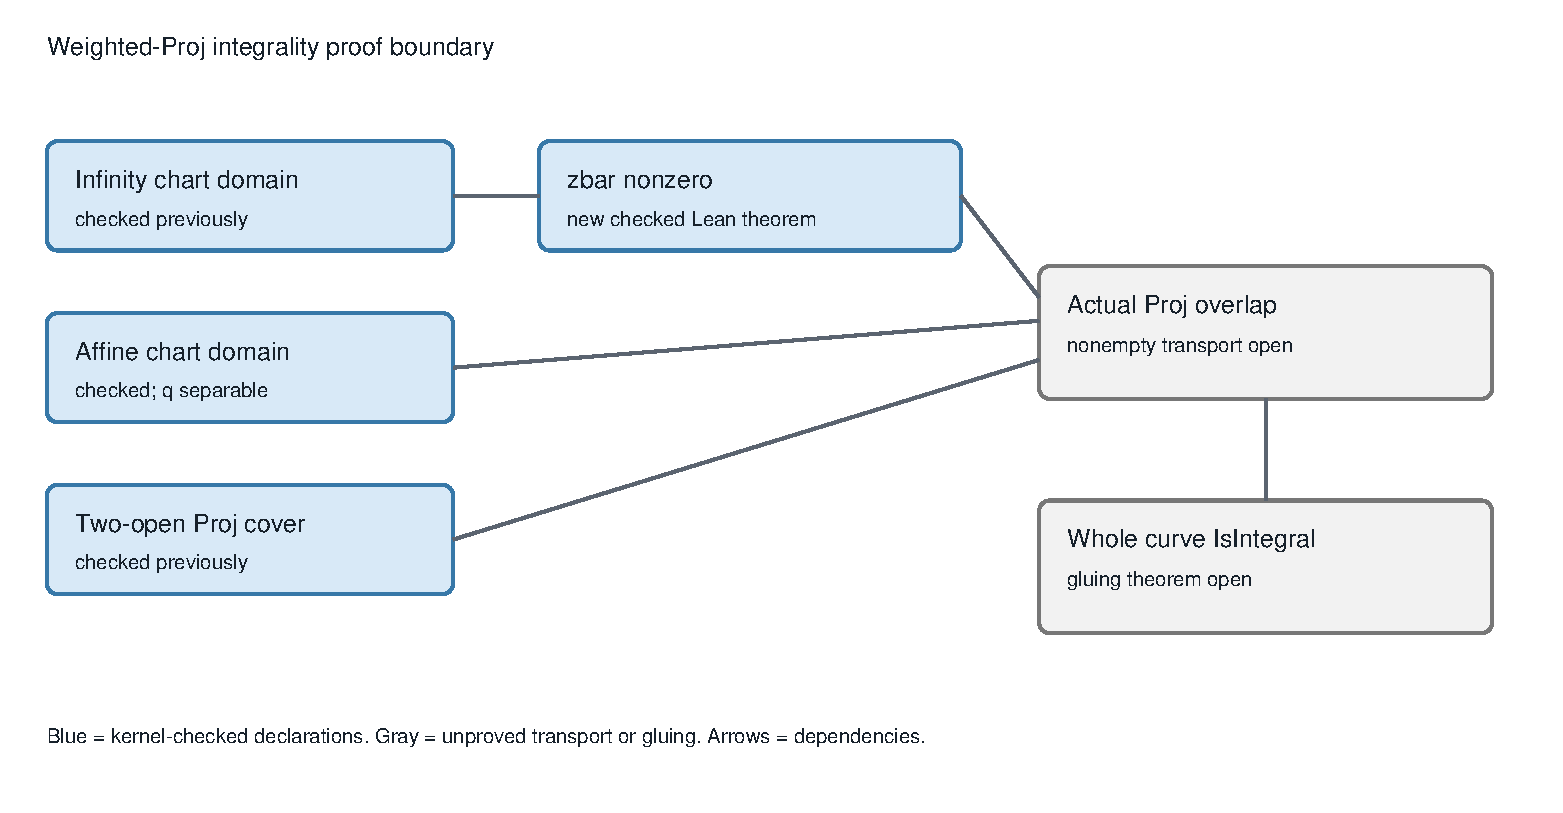
\includegraphics[width=0.96\textwidth,height=0.78\textheight,keepaspectratio]{projective-integral-figure.pdf}
\end{center}
\noindent Blue nodes are checked declarations; gray nodes are open. Arrows represent proof dependencies, not performance measurements.
\end{document}
